%%%%%%%%%%%%%%%%%%%%%%%%%%%%%%%%%%%%%%%%%
% Short Sectioned Assignment
% LaTeX Template
% Version 1.0 (5/5/12)
%
% This template has been downloaded from:
% http://www.LaTeXTemplates.com
%
% Original author:
% Frits Wenneker (http://www.howtotex.com)
%
% License:
% CC BY-NC-SA 3.0 (http://creativecommons.org/licenses/by-nc-sa/3.0/)
%
%%%%%%%%%%%%%%%%%%%%%%%%%%%%%%%%%%%%%%%%%

%----------------------------------------------------------------------------------------
%	PACKAGES AND OTHER DOCUMENT CONFIGURATIONS
%----------------------------------------------------------------------------------------

\documentclass[paper=a4, fontsize=12pt]{scrartcl} % A4 paper and 11pt font size

\usepackage[T1]{fontenc} % Use 8-bit encoding that has 256 glyphs
\usepackage{fourier} % Use the Adobe Utopia font for the document - comment this line to return to the LaTeX default
\usepackage[english]{babel} % English language/hyphenation
\usepackage{amsmath,amsfonts,amsthm} % Math packages
\usepackage{listings}
\lstset{basicstyle=\small\ttfamily, breaklines=truem}

\usepackage{lipsum} % Used for inserting dummy 'Lorem ipsum' text into the template
\usepackage{tikz}
\usepackage[]{graphicx}

\usepackage{sectsty} % Allows customizing section commands
\allsectionsfont{\centering \normalfont\scshape} % Make all sections centered, the default font and small caps

\usepackage{fancyhdr} % Custom headers and footers
\pagestyle{fancyplain} % Makes all pages in the document conform to the custom headers and footers
\fancyhead{} % No page header - if you want one, create it in the same way as the footers below
\fancyfoot[L]{} % Empty left footer
\fancyfoot[C]{} % Empty center footer
\fancyfoot[R]{\thepage} % Page numbering for right footer
\renewcommand{\headrulewidth}{0pt} % Remove header underlines
\renewcommand{\footrulewidth}{0pt} % Remove footer underlines
\setlength{\headheight}{13.6pt} % Customize the height of the header

\numberwithin{equation}{section} % Number equations within sections (i.e. 1.1, 1.2, 2.1, 2.2 instead of 1, 2, 3, 4)
\numberwithin{figure}{section} % Number figures within sections (i.e. 1.1, 1.2, 2.1, 2.2 instead of 1, 2, 3, 4)
\numberwithin{table}{section} % Number tables within sections (i.e. 1.1, 1.2, 2.1, 2.2 instead of 1, 2, 3, 4)

\setlength\parindent{0pt} % Removes all indentation from paragraphs - comment this line for an assignment with lots of text

\linespread{1.5}
%----------------------------------------------------------------------------------------
%	TITLE SECTION
%----------------------------------------------------------------------------------------

\newcommand{\horrule}[1]{\rule{\linewidth}{#1}} % Create horizontal rule command with 1 argument of height

\title{
\normalfont \normalsize
\textsc{EURECOM, Computation Methods for Digital Communication Systems} \\ [25pt] % Your university, school and/or department name(s)
\horrule{0.5pt} \\[0.4cm] % Thin top horizontal rule
\huge Fixed-point FFT Benchmarking \\ % The assignment title
\horrule{2pt} \\[0.5cm] % Thick bottom horizontal rule
}

\author{Simone Rossi} % Your name

\date{\normalsize\today} % Today's date or a custom date

\begin{document}

\maketitle % Print the title

%----------------------------------------------------------------------------------------
%	PROBLEM 1
%----------------------------------------------------------------------------------------

\section{Introduction}

In this laboratory, we studied the effects of fixed-point representation for a
well known algorithm in Digital Signal Processing, the \textbf{FFT}, a fast algorithm
for computing the DFT of a signal.

\section{Fixed-point operation routines}

Let's analyze how fixed-point numbers are represented and how we can emulate
arithmetic operations with them.

\subsection{Multiplication in Q15}

This is the code for implementing a multiplication with two operands in Q15.

\lstinputlisting[firstline=1,lastline=3, language=C]{code/fixed_point.c}

Simply, it casts both operands in 32 bit integers, performs the multiplication and
takes the most significant bits of the result by shifting to the right of
15 positions. Before returning, the result is casted back to \texttt{short}.

\subsection{Multiplication for Q25 $\times$ Q18}

Here the situation is slightly different but the procedure is similar: operands
are casted in 64 bits (to avoid overflow issues) and the right most 25 bits are
taken as result.

\lstinputlisting[firstline=14,lastline=16, language=C]{code/fixed_point.c}


\subsection{Saturated addition in Q15 and Q25}

This is the code for implementing a saturated addition with two operands in Q15.

\lstinputlisting[firstline=5,lastline=12, language=C]{code/fixed_point.c}

It extends the operands on 32 bits and it checks whether the result will be an
overflow or not. If so, it returns the maximum number representable on 16 bits
($2^{16}-1 = 32767$), positive or negative according to the case. If not, it simply
returns the normal sum.\\

For the operation in Q25, the procedure is exactly the same with the exception
of the return value in case of overflow, which is now $2^{24}-1$

\lstinputlisting[firstline=18,lastline=25, language=C]{code/fixed_point.c}

\subsection{4-point Butterfly in Q15}
This is the code I modified for computing the simulated results in Q15.
\lstinputlisting[firstline=28,lastline=44, language=C]{code/fixed_point.c}

\subsection{4-point Butterfly in Xilinx DSP format}
This is the code I modified for computing the simulated results in the Xilinx DSP format.
\lstinputlisting[firstline=47,lastline=63, language=C]{code/fixed_point.c}

\section{Twiddle factor quantization}

\begin{minipage}{.4\textwidth}
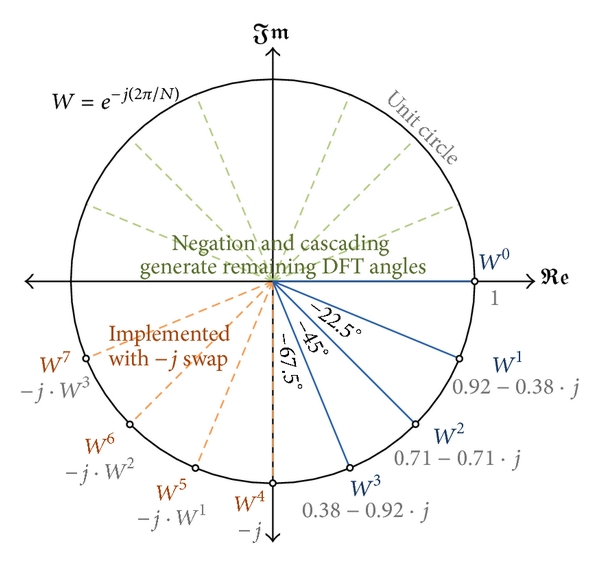
\includegraphics[width = \textwidth]{fig1.jpg}
\end{minipage}
\hspace{.5cm}
\begin{minipage}{.6\textwidth}
Generally twiddle factors are chosen such that the lay in the unity circle in
the complex domain and it's written as
\begin{equation}
    \textbf{W}_i = \left[ \cos(i2\pi/N), -\sin(i2\pi/N) \right]
\end{equation}
However this might not always be the case when we deal with
quantization and fixed point representation.
\end{minipage}
What is currently done is to take always the \texttt{floor} value for the sine
and cosine; another possible strategy for computing the twiddle factor could be
calculating all four possible combinations of approximations and taking the one
which is less distant from the unity circle.

\section{Distortion test}
The distortion test is computed as follows.
\begin{equation}
    \bar x^{in} = \sum_{i=0}^{N-1}\left[ \Re\left\{ x^{in}_i \right\}^2 +
                                         \Im\left\{ x^{in}_i \right\}^2 \right]
\end{equation}
\begin{equation}
    \bar \epsilon = \sum_{i=0}^{N-1}\left[  \Re\left\{ x^{in}_i - \dfrac{x^{FP}_i}{2^{16}-1} \right\}^2 +
                                            \Im\left\{ x^{in}_i - \dfrac{x^{FP}_i}{2^{16}-1} \right\}^2 \right]
\end{equation}

\begin{equation}
    SNR = 10\log_{10}\dfrac{\bar x^{in}}{\bar \epsilon}
\end{equation}

This is the code for doing so.

\lstinputlisting[firstline=65,lastline=73, language=C]{code/fixed_point.c}

This benchmarking has been performed on three signals. The first test is with a
sinusoidal input. The second a random 16-QAM signal as input and finally the third
is a white-noise signal.

\section{Results}
These are the results I got in the two cases. The first one is the traditional
Q15 format.

\begin{minipage}{.5\textwidth}
    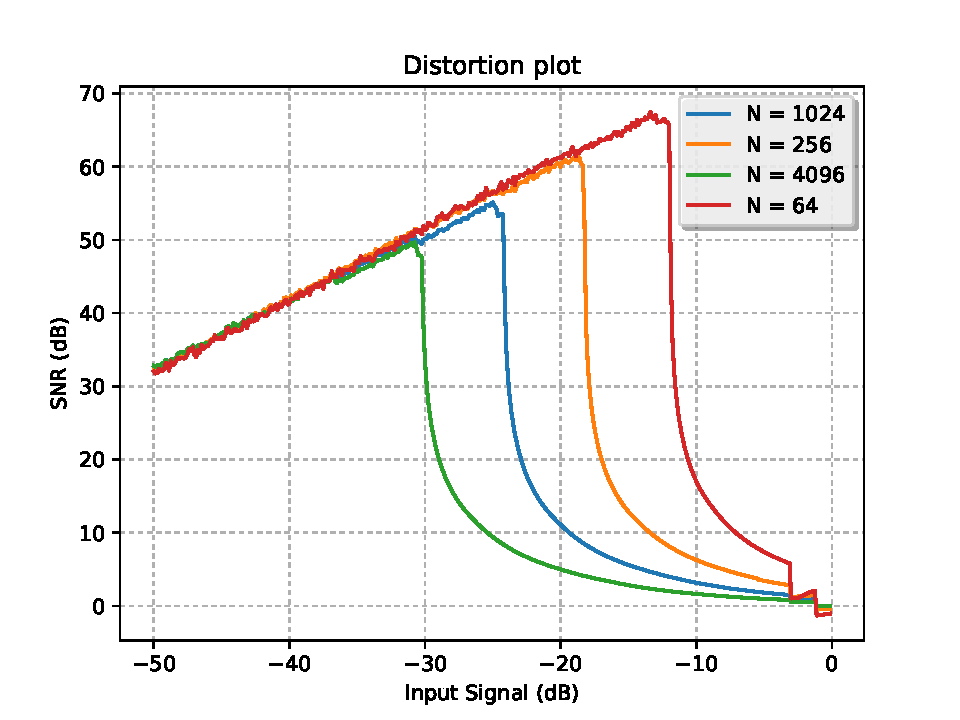
\includegraphics[width = \textwidth]{../figQ15/TEST_0.pdf}
\end{minipage}
\begin{minipage}{.5\textwidth}
    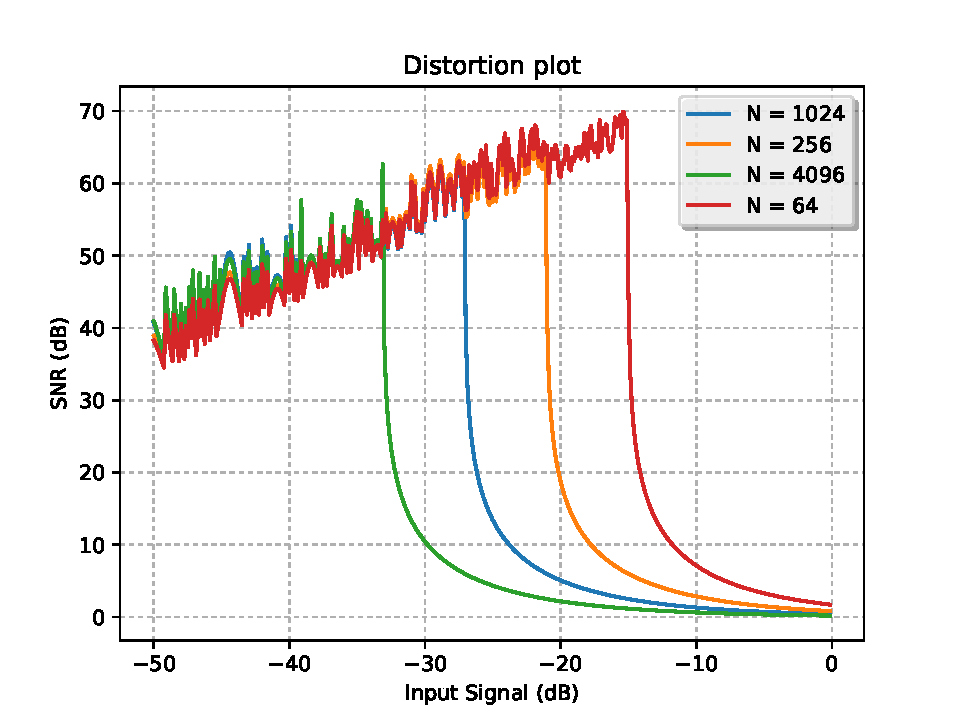
\includegraphics[width = \textwidth]{../figQ15/TEST_1.pdf}
\end{minipage}

\begin{minipage}{\textwidth}
    \centering
    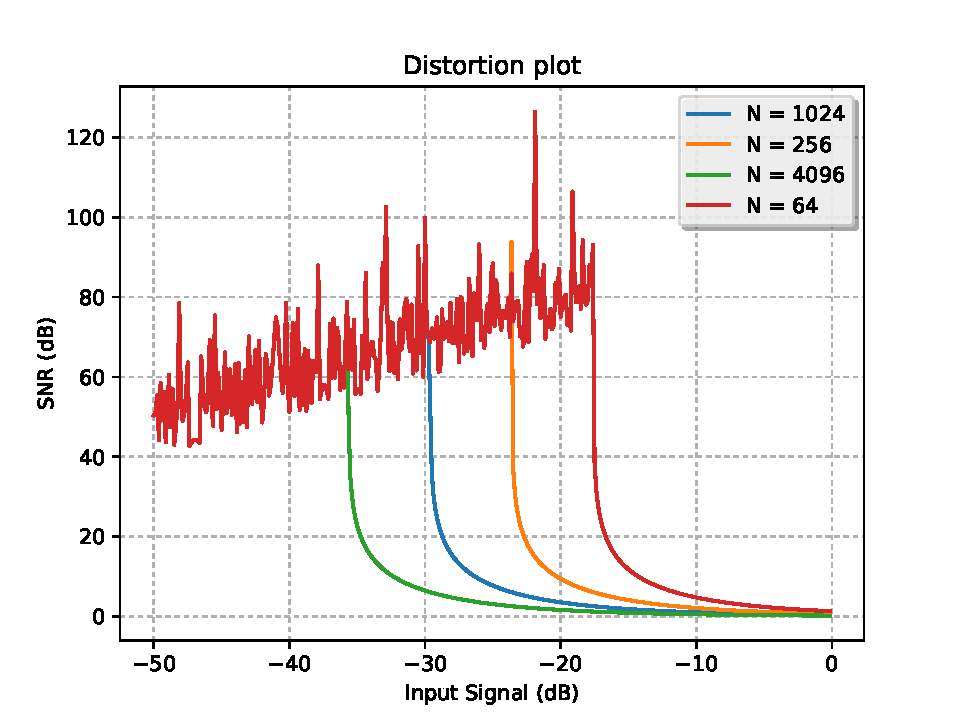
\includegraphics[width = 0.5\textwidth]{../figQ15/TEST_2.pdf}
\end{minipage}

As we can see, in all the three tests, the system suffers performance degradation
when the input signal power starts to become higher and higher, possibly due to
overflow/underflow in some butterfly stage. As expected, the lower the
number of FFT points, the higher is the breakdown point.\\

The following one, on the other hand, is the one with the Xilinx DSP format.

\begin{minipage}{.5\textwidth}
    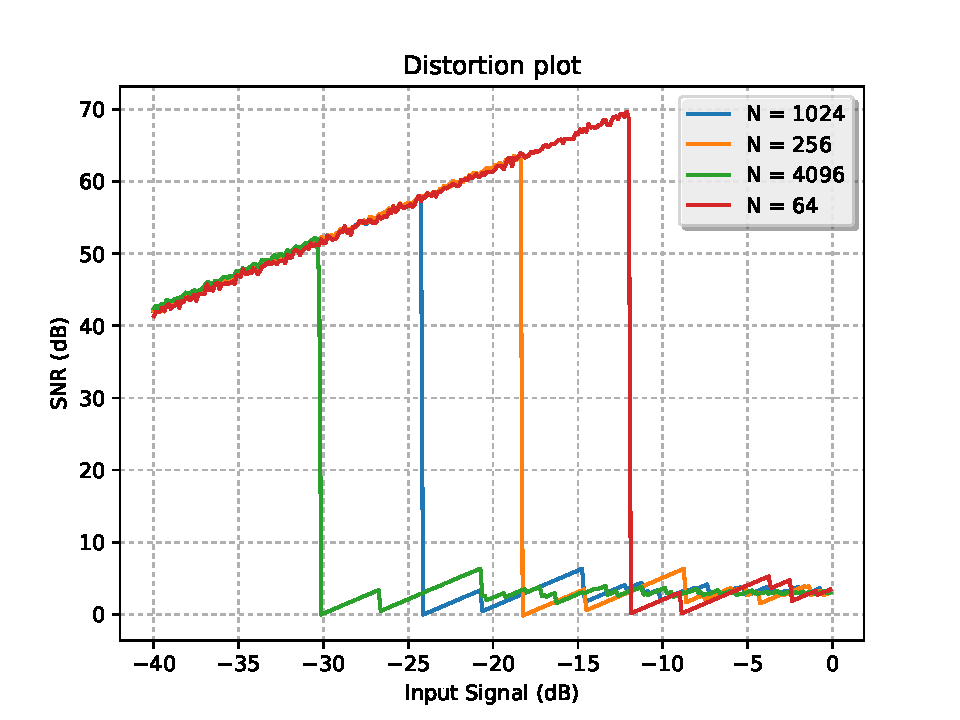
\includegraphics[width = \textwidth]{../figQ24/TEST_0.pdf}
\end{minipage}
\begin{minipage}{.5\textwidth}
    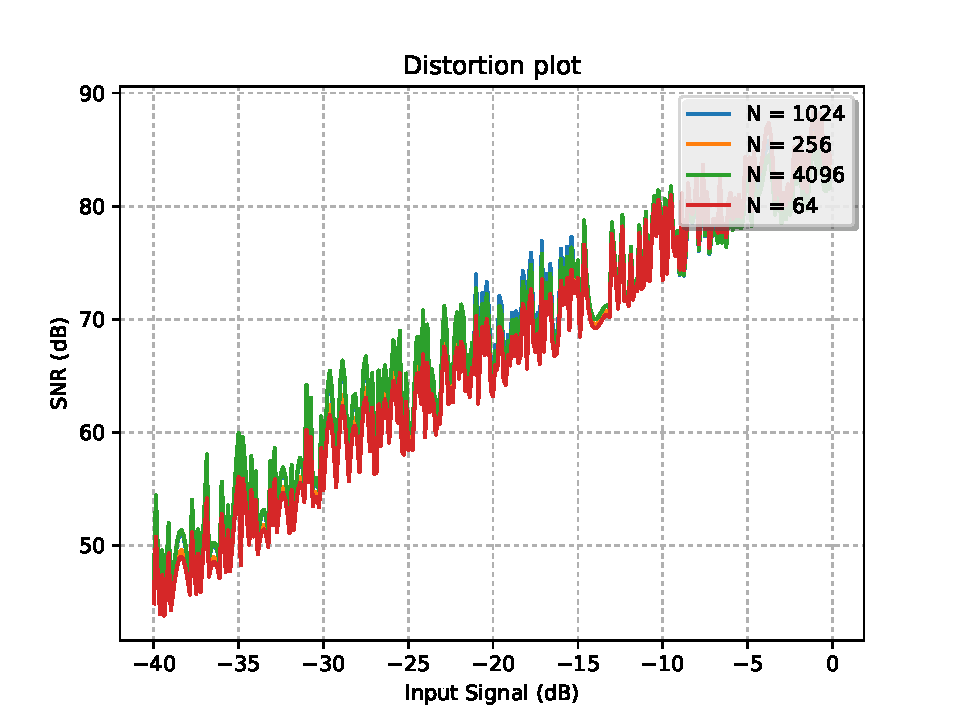
\includegraphics[width = \textwidth]{../figQ24/TEST_1.pdf}
\end{minipage}

\begin{minipage}{\textwidth}
    \centering
    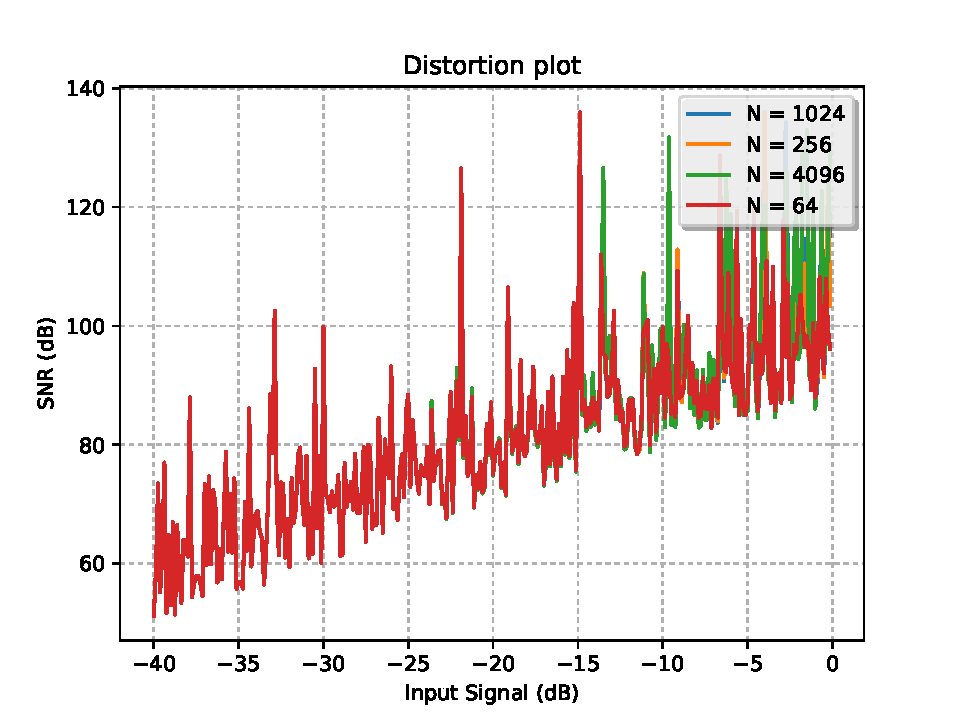
\includegraphics[width = 0.5\textwidth]{../figQ24/TEST_2.pdf}
\end{minipage}

With sinusoidal input, the behaviour is not so different from the Q15 but the results for
the other two tests is interesting. It seems that this particular format for fixed point
can avoid destructive overflows.

\end{document}
